% Part: biographies 
% Chapter: ernst-zermelo
% Section: biography
\documentclass[../../../include/open-logic-section]{subfiles}

\begin{document}

\olfileid{bio}{erz}{bio} 
\olsection{Biography}

\begin{figure}[h!] 
\centering
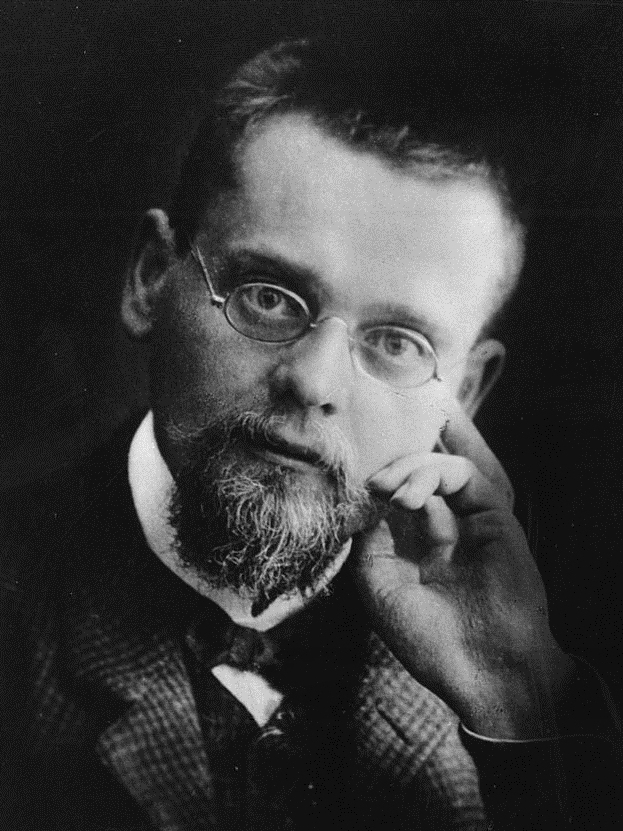
\includegraphics[scale=0.5]{ernst-zermelo.jpg} 
\caption{Ernst Zermelo. Photo Credit: Wikimedia Commons.} 
\end{figure}
Ernst Zermelo was born on July 27, 1871 in Berlin, Germany. He had five sisters,
though his family suffered from poor health and only three made it to adulthood. 
His parents also passed away when he was young, leaving him and his sibilings
orphans when he was seventeen. Although known
as a mathematician, Zermelo had an interest in the arts, and especially in poetry
\citep[5]{ebbinghaus2015}. Known for being 
sharp, witty, and critical, Zermelo also had a softer side. 


Zermelo's interests at univeristy were varied. He took courses in physics, 
mathematics, and philosophy, including attending lectures by Georg Cantor
and Edmund Husserl, David Hilbert and Felix Klein. Under the supervision of Hermann Schwarz, Zermelo
completed his dissertation
\emph{Untersuchungen zur Variations-Rechnung (Investigations
In the Calculus of Variations)} on theoretical physics in 1894 at the University of Berlin.
In 1897, he decided to pursue more studies at the Univeristy of G\"{o}ttigen where he
was heavily influenced by the work of David Hilbert and Felix Klein. He began to publish 
in set theory at the beginning of the twentieth century. He is perhaps best known for
 the axiomatization of set theory, and for formulating the axiom of choice.
 
 He filed for two patents, and was among the first to propose an automatic gear shifting
 mechanism for automobiles \citep[155]{ebbinghaus2015}.
  In 1921 Zermelo moved to Freiburg where he taught as an honourary professor
  at the Univeristy of Freiburg. In 1931 he submitted an unsuccessful patent application
  for an instrument that stabilized bicycles during a stop while providing energy for
  starting up again \citep[154]{ebbinghaus2015}. During his time at Freiburg, Zermelo
  got caught up in controversy with both Thoralf Skolem and Kurt G\"{o}del. 

\end{document}